%!TEX root = ../thesis.tex
%*******************************************************************************
%****************************** Introduction Chapter ***************************
%*******************************************************************************
\chapter{Background}

This thesis examines graph genome methods and their application to bacterial genomes. In particular, we focus our attention on \textit{Mycobacterium tuberculosis} and \ont{} sequencing for these applications. 

We begin with the concept of a bacterial pan-genome and discuss the limitations of current approaches for its interrogation. Next, we introduce graph genomes as a more intuitive model for investigating the bacterial pan-genome. We then provide more detail on a particular genome graph method, Pandora, a focal point in the ensuing chapters. A survey of nanopore-based sequencing is then provided, motivating its use as the primary source of genomic data in this thesis. Finally, we introduce tuberculosis (TB) and its causative pathogen, \mtb{}. We outline the global effort to end TB and discuss the diagnostic challenges we address in this thesis.

% =============================================
\section{Bacterial genomes}

\subsection{Drivers of bacterial diversity}

Bacteria have incredibly flexible genomes. Their mechanisms of variation can be grouped into \emph{vertical} or \emph{horizontal} inheritance. Vertical inheritance is the passing of genetic material from parent to offspring during replication, while horizontal inheritance describes the acquisition of genetic information between cells without such an ancestor relationship. 

Vertically inherited variation generally consists of genetic point mutations, insertions and deletions (indels), and structural rearrangements. Such mutations can arise due to a multitude of reasons: homologous recombination, DNA deamination, replication-transcript conflict, and replication errors, to name a few \cite{Lan2000}. However, the dominant form of genomic variability in bacteria is horizontal inheritance \cite{McInerney2017}.

Horizontal inheritance operates via the three main mechanisms \emph{transduction}, \emph{conjugation}, and \emph{transformation}. These are illustrated in \autoref{fig:horizontal-inheritance}.

\emph{Transduction} is mediated by bacteriophages (phages) - viruses which infect bacteria and are the most abundant organism on Earth \cite{mcgrath2007bacteriophage}. During phage propagation, parts of the host (bacteria) DNA can become encapsulated in the virus. If a phage goes on to infect another cell and eject this encapsulated DNA (transduction), it can recombine into the chromosome or begin replicating as a plasmid \cite{Chiang2019}. When the transduced DNA is a gene that imparts a new, beneficial function, it can impact the recipient's evolution.

\emph{Conjugation} is the cell-to-cell transfer of DNA. A donor cell contacts another via a pilus, and a copy of the DNA - usually a plasmid - is transmitted \cite{Soucy2015}. A rarer form of conjugation can occur when a plasmid has become incorporated into the chromosome of the donor (Hfr), and this portion of the chromosome is transferred to the recipient cell \cite{Redfield2001}.

\emph{Transformation} occurs when a cell internalises exogenous DNA, which in turn becomes incorporated into the chromosome by homologous recombination \cite{Johnston2014}. There is some debate about the exact purpose of transformation, with the consensus being it increases genetic diversity; however, a nutritional role is also a possibility \cite{Johnston2014}.

\begin{figure}
\begin{center}
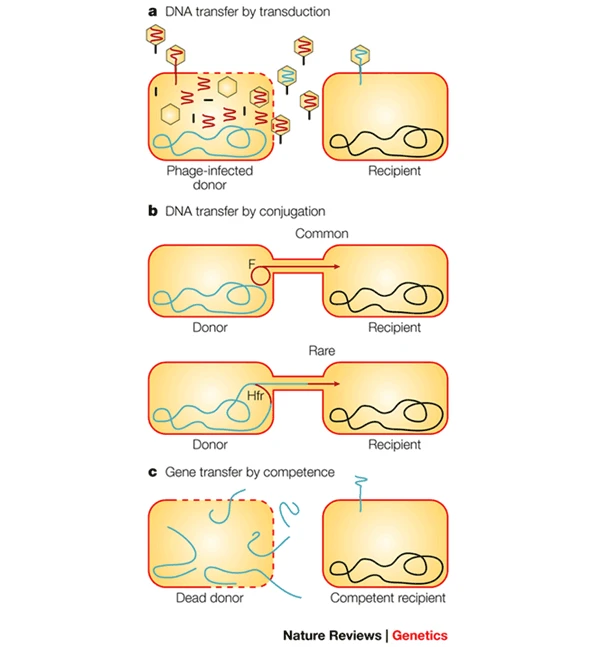
\includegraphics[width=0.8\columnwidth]{Chapter0/Figs/methods-of-dna-transfer.png}
\caption{{An illustration of the three main mechanisms of horizontal inheritance in bacteria. \textbf{a}) Transduction is facilitated by phages that encapsulate host DNA in one cell and eject that DNA into another cell. \textbf{b}) Conjugation, in its prevalent form, is the transfer of a plasmid copy from a donor to a receiver cell via a pilus "bridge". In a rarer form, a plasmid that has been incorporated into the donor cell chromosome is transferred. \textbf{c}) Transformation (competence) is the uptake of exogenous DNA and subsequent incorporation into the chromosome.}
{\label{fig:horizontal-inheritance}}
}
\source{\cite{Redfield2001}}
\end{center}
\end{figure}

\noindent
These different means of inheritance compound to create varying diversity levels within bacterial species and give rise to the \emph{pan-genome}.

\subsection{The pan-genome}

A pan-genome is the full complement of genetic loci found within a given species. Traditionally, loci refer to genes, although we note that loci need not be genes for the work we will describe in this thesis.

The pan-genome can be broken into two subsets: the \emph{core} and \emph{accessory} genome. Loci that occur in the majority of species members are considered core, whilst everything else is deemed accessory (see \autoref{fig:pangenome-venn}). The accessory genome can be further divided into intermediate and rare loci. 

The proportional size of the core genome varies dramatically between species. For instance, if we assume a gene is core when present in $\ge 95$\% of sampled species, the \textit{Escherichia coli} pan-genome is composed of 10\% core genes. Conversely, 89\% of the \textit{Mycobacterium tuberculosis} pan-genome is core genes (data was obtained from the panX database \cite{panx}). Species with a large pan-genome, such as \ecoli{}, have what is called an "open" pan-genome, while those with more conserved gene content, such as \mtb{}, are deemed "closed". 

Another interesting property of the bacterial genome is the distinctive "U-shaped" gene frequency distribution \cite{Lobkovsky2013,pandora,Lapierre2009}, shown in \autoref{fig:pangenome-freq}. This frequency distribution is a consequence of the fact that, in general, genes are either rare or common due to selective pressures \cite{Lobkovsky2013,thepangenome2020}. Moreover, the size of the bacterial pan-genome is estimated to be infinite \cite{Lapierre2009}, as hinted at by \autoref{fig:pangenome-size}.

\begin{figure}
     \centering
     \begin{subfigure}[b]{0.475\textwidth}
        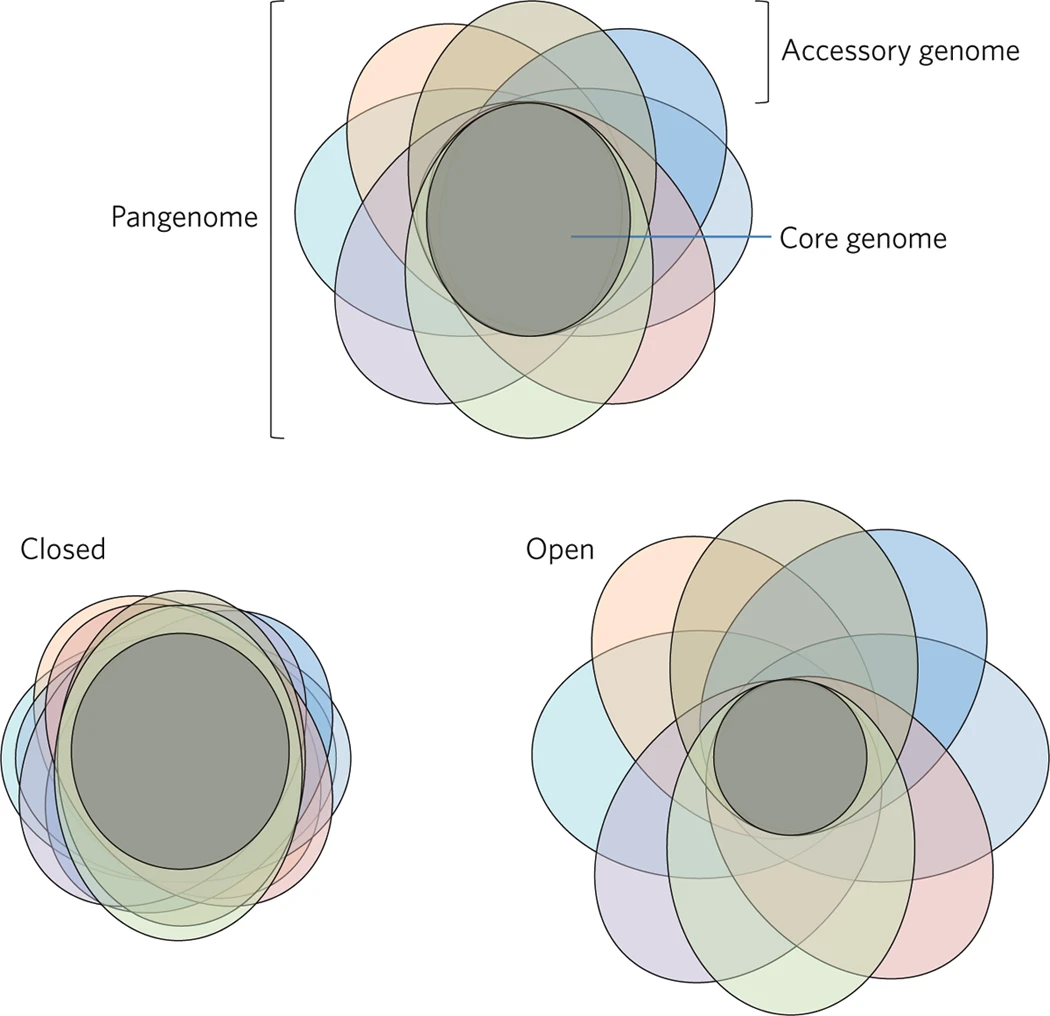
\includegraphics[height=0.21\textheight]{Chapter0/Figs/pangenome-venn.png}
        \centering
        \caption{}
        \label{fig:pangenome-venn}
        \source{\cite{McInerney2017}}
     \end{subfigure}
     \begin{subfigure}[b]{0.475\textwidth}
         \centering
        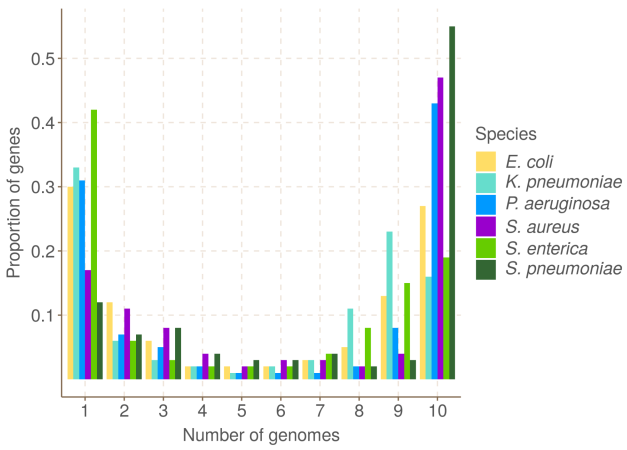
\includegraphics[height=0.21\textheight]{Chapter0/Figs/gene_frequency_distribution.png}
         \caption{}
         \label{fig:pangenome-freq}
         \source{\cite{pandora}}
     \end{subfigure}
     \begin{subfigure}[b]{0.8\textwidth}
        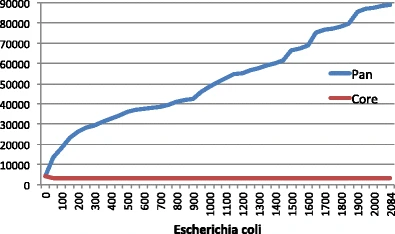
\includegraphics[width=1\linewidth]{Chapter0/Figs/pangenome-size.png}
        \centering
        \caption{}
        \label{fig:pangenome-size}
        \source{\cite{Land2015}}
     \end{subfigure}
    \caption{The size and gene frequency distribution of the bacterial pan-genome. \textbf{a}) Venn diagram representation of the pan-genome and its core and accessory components. \textbf{b}) The asymmetric U-shaped gene frequency distribution for 10 genomes within 6 bacterial species. Genes are generally rare (left) or common (right). \textbf{c}) the size (y-axis) of the core (red) and accessory (blue; Pan) genome of \ecoli{} as more genomes are sampled (x-axis).}
        \label{fig:pangenome}
\end{figure}

\noindent
These definitions of the pan-genome components (core and accessory) are somewhat simplistic. Recent work by Horesh \etal{} has highlighted that these traditional definitions are biased by lineage sampling \cite{Horesh2021}. For example, we have a collection of 100 genomes, with 50 being from the same lineage ($L_1$). Let us say gene \textit{abc} occurs in all 50 members of $L_1$, but none of the other 50 genomes. Under the traditional pan-genomic definitions, we would call \textit{abc} an intermediate accessory gene. However, if we gathered a further 1,000 genomes, none of which are lineage $L_1$, \textit{abc} would now be considered rare. In the new pan-genome model proposed by Horesh \etal{}, loci are given a classification that is structure-aware. The \textit{abc} gene from our example would be classified as "lineage-specific core", acknowledging the fact that the sampled lineages in a collection provide essential contextual information. Other categories include multi-lineage and collection core and the same categories for intermediate, rare, and a new varied frequency class. The collection core is analogous to the traditional core, with everything else being the accessory genome - albeit with a much finer level of detail.

\subsection{How are pan-genomes analysed?}
\label{sec:analyse-pangenome}

Most pan-genomic analyses of bacterial collections follow a similar approach: align the genomes with a tool such as Parsnp \cite{Treangen2014} or Rory \cite{Page2015}, extract the core genome alignments and either ignore the accessory genome or produce a presence-absence matrix of it \cite{Arnold2018,Azarian2018,McNally2016,thepangenome2020}. When the accessory genome is investigated at the nucleotide level, it is generally focused on a small subset of genes related to specific phenotypes such as antimicrobial resistance (AMR; \cite{Boolchandani2019}) or virulence \cite{Vasquez2019}. However, as we have seen, the pan-genome size varies significantly, so depending on the species, such approaches could be "ignoring" large portions of the total genomic repertoire. Despite this, we have learned an enormous amount about bacteria and their pan-genomes with these methods.

\subsection{Variant calling of bacterial genomes}
\label{sec:intro-bacteria-var-call}

A typical (pan-)genomic analysis requirement, and a focus of this thesis, is variant calling. However, depending on the application, this can be done in many different ways. For example, when characterising an outbreak, common approaches are to use a reference genome of the same, or very close, strain to the outbreak \cite{Taylor2015}, or assemble each sample and select the closest reference to it based on some typing strategy \cite{Wyres2021}. Alternatively, a reference-free approach can alleviate some of the reference bias induced when selecting a genome to call variants against and provide better resolution of an outbreak \cite{Cremers2020}.

Given the importance of bacterial variant calling to this thesis, we will briefly outline various approaches to calling variants in bacterial genomes and highlight their strengths and limitations.

\subsubsection{Alignment-based methods}
\label{sec:aln-var-call}
Alignment-based variant calling requires a reference genome. In this mode of variant calling, raw sequencing reads are aligned to a given reference genome to generate a Sequence Alignment/Map (SAM) file. Common software programs used to perform these alignments for bacterial variant calling include BWA-MEM \cite{li2013}, Bowtie2 \cite{bowtie2012}, and Novoalign (\url{http://www.novocraft.com/products/novoalign}) for short (Illumina) read technology. (\ont{}-based variant calling will be detailed in \autoref{sec:ont-var-calling-intro}, for now we focus on Illumina-based sequencing reads). 

Where variant calling programs distinguish themselves is in how they handle the alignment information. This includes, but is not limited to, the number of base calls disagreeing with the reference, the quality of the read alignment, the alignment locations of a read pair, or the quality score of the mapping \cite{Olson2015}. Popular methods for calling variants generally employ either Bayesian, likelihood, or machine learning algorithms to infer candidate variants given this alignment data. While many of these models were designed for human variant calling, a selection have shown themselves to be perfectly applicable to bacteria. The most frequently used Bayesian method for bacterial variant calling is Freebayes \cite{Garrison2012}; however, it is generally used via a wrapper, Snippy (\url{https://github.com/tseemann/snippy}), which handles the alignment (BWA-MEM), variant calling (Freebayes), and additionally applies filters to the resulting VCF file. Of the likelihood-based callers, Samtools/BCFtools \cite{bcftools2021,samtools2009} and GATK \cite{Poplin2018} tend to be most often employed. 

\subsubsection{Alignment-free methods}
In general, methods that do not align reads to a reference genome use \kmer{}-based algorithms for variant inference. FastGT \cite{fastgt2017} and LAVA \cite{lava2016} are two such programs that require a database of known variants and use \kmer{} counts in a sample to determine the presence of any of these variants. The major limitation with these tools is their inability to call variants not present in the provided database. Kestrel \cite{kestrel2017} is a \kmer{}-based variant caller that can \denovo{} discover variants and does this by detecting unique \kmer{}s in a sample, with respect to a given reference genome. However, Kestrel is not strictly alignment-free, as it does use local alignment to place candidate variants in relation to the reference genome. Additionally, it was shown to have much lower sensitivity than alignment-based methods. 

Another popular alignment-free single nucleotide polymorphism (SNP) caller is kSNP, which finds SNPs \emph{between} samples by detecting \kmer{}s where the central base varies \cite{ksnp2015}. It is regularly used in outbreak settings where differences between samples are crucial \cite{Bazan2017,Raphael2016,Chochua2017}. However, kSNP cannot detect SNPs within $k$ positions (bases) of each other or detect indels, and cannot deal with sequencing errors - requiring extensive pre-filtering.

A benchmark of alignment-free methods for various sequence analysis applications can be found in \cite{Zielezinski2019}. 

\subsubsection{Assembly-based methods}
\label{sec:asm-var-call}
There are two forms of assembly-based variant calling. In the first, an assembled genome for a sample (or samples) is compared to a reference via whole-genome alignment. Software such as MUMmer \cite{mummer2018} or Minimap2/paftools \cite{li2018} facilitate this assembly-to-assembly alignment and then identify positions where the two disagree. An assembly-based method that is prevalent in bacterial genomics is Parsnp \cite{Treangen2014}, which aligns the \emph{core} genome of assemblies and then calls SNPs (only) \emph{between} those genomes. A major limitation with these types of assembly-based approaches is that there is no sense of the quality of calls. As an assembly naturally has a depth of 1x at all positions, there is no information about variant support - all variants are considered equal in this scheme.

The second form of assembly-based variant calling performs assembly and genotyping. Cortex \denovo{} assembles a sample from sequencing reads and genotypes variants at "bubble" sites in its de Bruijn graph \cite{iqbal2012}. It produces variant calls with respect to a provided reference genome and has been used extensively in bacterial genomics \cite{bradley2015,hunt2019,Stasiewicz2015,Young2017,Lees2017}.

\hspace{0.75cm}

\noindent
A recent comprehensive benchmark of alignment-based variant calling found that the choice of reference genome, rather than the choice of tools, has the most critical impact on accuracy \cite{Bush2020}. The best general-purpose pipeline was found to be Snippy; however, they note that species-specific filtering of the final VCF file can cause the performance of many tools to converge.

Reference genome bias is the most significant limitation of bacterial variant calling approaches \cite{Bertels2014,Bush2020,Olson2015}. The bacterial pan-genome highlights this impediment in a stark way. As an illustration of this, \autoref{fig:reference-bias} shows a cartoon depiction of the "single-reference problem". In this figure, we see that no two genomes contain the same complete set of loci - precisely what we expect from nearly any pan-genome \cite{McInerney2017}. Thus, using any of these genomes as a reference to call variants against will inevitably mean we cannot describe variants in loci not found in both the reference and query genomes. This type of bias is termed \emph{hard} reference bias. Another, more subtle, form is \emph{soft} reference bias, which results from difficulties aligning to the reference due to divergence in shared loci between the reference and query - especially around structural variants \cite{Price2017,Olson2015,Pightling2014}. However, these biases tend to impact clonal species, such as \mtb{}, much less than those with open pan-genomes \cite{Bush2020}.

\begin{figure}
\centering
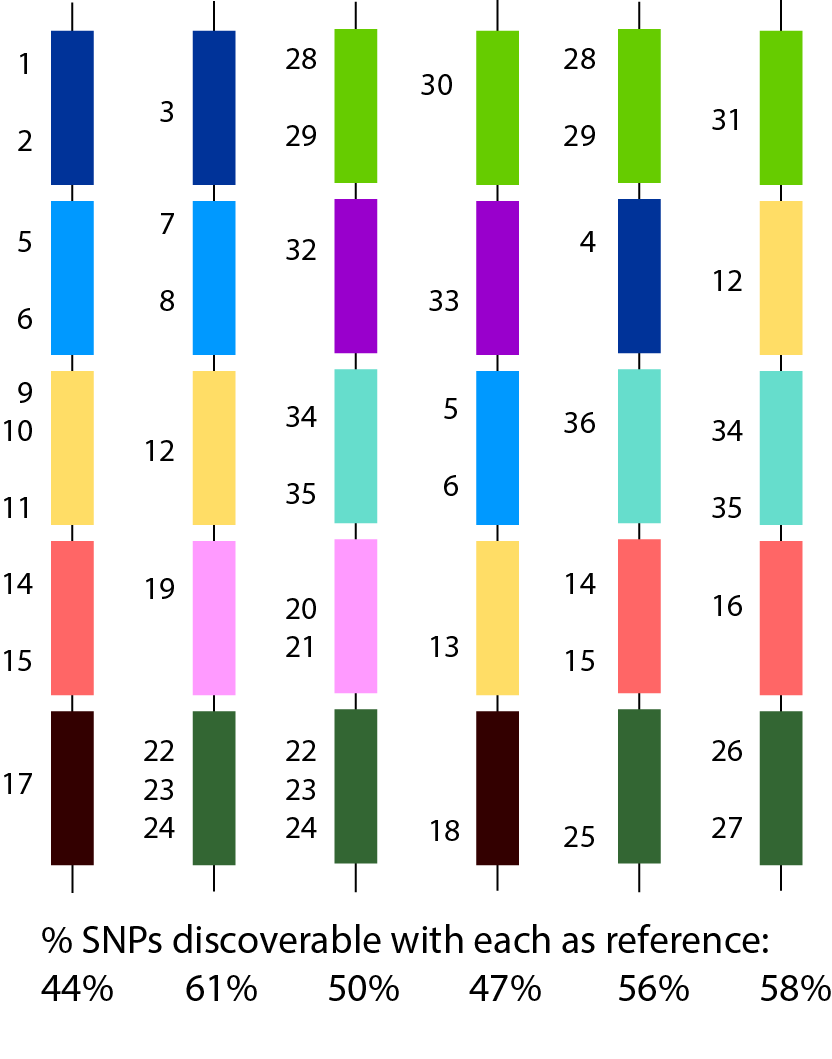
\includegraphics[height=0.35\textheight]{Chapter0/Figs/single_ref_problem.png}
\caption{An illustration of the single-reference problem. Each vertical column depicts a genome, with the coloured blocks representing loci (genes). The numbers next to each locus indicate a variant with respect to other loci of the same colour. The percentage figures at the bottom indicate what percentage of variants in the other genomes could be found by a perfect variant caller if that genome was used as a reference. Not all genomes contain the same loci; hence no genome can capture all of the variants.}
\label{fig:reference-bias}
\source{\cite{rachelthesis,pandora}}
\end{figure}

Given the biases resulting from the use of a single reference genome, an alternative solution is needed. One solution that is rapidly maturing is the use of a \emph{genome graph} to replace a single reference.

% =============================================
\section{Genome graphs}

Genome graphs are a way of representing variation within a population; be it a bacterial species, a human gene, or a viral quasi-species \cite{comp-pan-genomics}. \autoref{fig:graph-representation} illustrates a generic representation of a genome graph, where redundant information (consensus) is collapsed into a linear sequence and variation is represented as divergent paths leading in and out of these linear segments. A walk through such a graph represents a mosaic of the population variation used to construct the graph. 

A rich array of algorithms and methods have been proposed for representing and operating on genome graphs across all kingdoms of life \cite{Sherman2020,Eizenga2020,comp-pan-genomics}. In this section, we will highlight some mature genome graph frameworks, along with their limitations. In the context of this thesis, these limitations will focus on the applicability of a method to the bacterial pan-genome. We follow these existing methods by introducing a new genome graph approach relevant to this thesis.

\begin{figure}
\centering
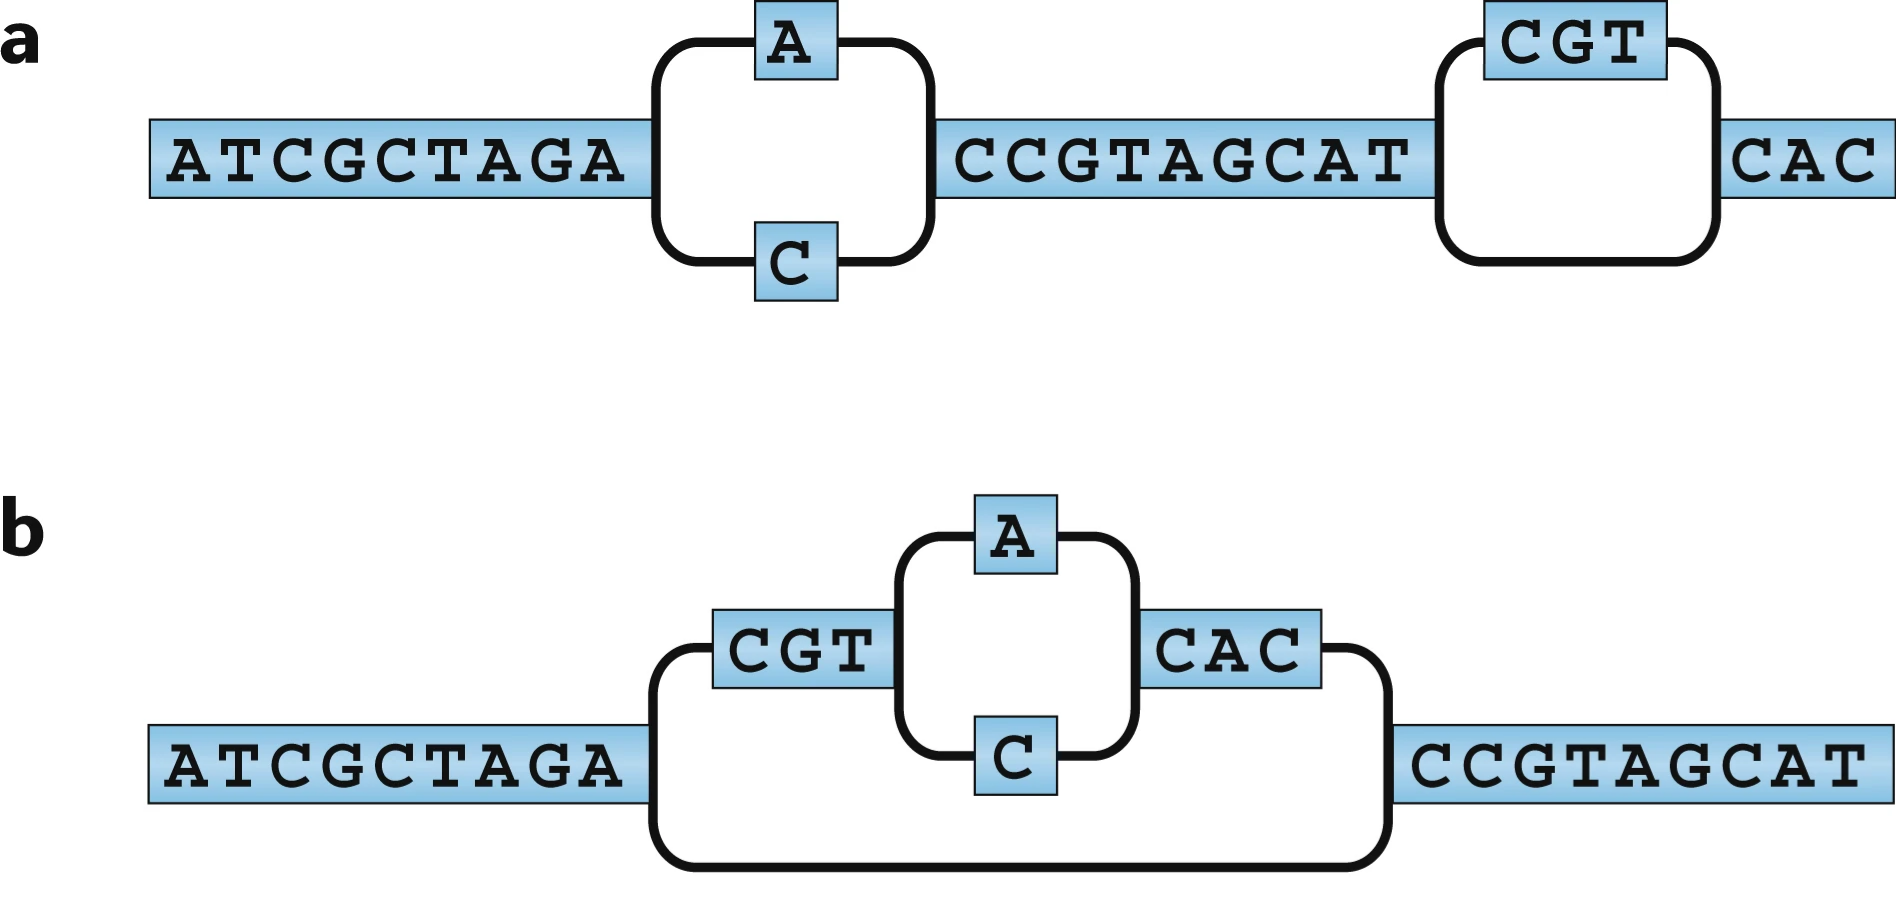
\includegraphics[width=0.75\columnwidth]{Chapter0/Figs/graph-representation.png}
\caption{Conceptual representation of a genome graph. \textbf{a}) Variants lead to a "bubble", or divergent path. Note, the second bubble represents an insertion/deletion. \textbf{b}) Variation can be arbitrarily nested. In this example, there are is a SNP within an insertion.}
\label{fig:graph-representation}
\source{\cite{Sherman2020}}
\end{figure}

\subsection{Existing methods}
\label{sec:graphs-existing}

\subsubsection{GraphTyper}
GraphTyper \cite{graphtyper,graphtyper2} represents a genome graph as a directed acyclic graph (DAG) based on a reference sequence plus known variants (similar to \autoref{fig:graph-representation}, but with directional). Sequencing reads are mapped to the reference genome with BWA-MEM. The reference sequence is then broken into 50kbp regions and reads are realigned to the graph in the respective region they map to. A path through the graph for the read is detected using a seed-and-extend approach and variants are genotyped based on the read support from this alignment. Impressively, GraphTyper can genotype SNPs, indels, and complex and structural variants.

In the context of bacterial genomes, there are a number of limitations with GraphTyper. First, a single reference genome is used as the backbone of the graph; a feasible solution for humans, but not for bacteria, where, as we have seen, two genomes likely do not have an identical gene repertoire. Second, the initial alignment of reads to the single reference genome suffers the same soft and hard reference bias discussed in \autoref{sec:intro-bacteria-var-call}. The realignment of reads reduces the soft reference bias compared to linear genome methods, however the hard bias remains. Third, no long-read sequencing technology support is available, and is unlikely to be possible with the current seed-and-extend approach used for alignment \cite{li2018}. 

\subsubsection{Variation graph toolkit}
The Variation Graph Toolkit (VG) \cite{vg2018} is a suite of tools for constructing, mapping, and calling variant from genome graphs. The representation used by VG is an \emph{un}directed, potentially cyclic, graph. Variation graphs can be constructed from a single reference and associated VCF file, or from multiple genome assemblies. Read alignment to the graph uses a seed-and-extend approach. Variant calls are made via a basic read pileup on the graph and then augmenting the original graph with novel candidates, followed by genotyping \cite{Novak2017}.

As with GraphTyper, the use of seed-and-extend alignment makes the support of long reads unlikely. (We note there has discussions within the VG GitHub repository for 4 years about supporting long reads, however, as yet, no support has been announced). Another limitation of VG is that in order to produce variant calls, the user must provide a reference genome, again, either inheriting reference bias or requiring a verbose description of simple variants (see \autoref{sec:pandora-compare} for an elaboration of this point).

A major limitation of VG is its computational resource requirements. As VG attempts to be a "general" method - i.e., it is undirected and allows cycles so as to naturally allow events such as inversions and repeats - it is CPU and disk intensive \cite{strainflair2021,gramtools2021,minigraph2020} to the point of requiring over 1 terabyte of temporary disk space to construct a graph \cite{gramtools2021}, or not being useable \cite{minigraph2020}.

\subsubsection{Minigraph}
Minigraph \cite{minigraph2020} represents a genome graph as a bidirectional graph, which allows cycles. The construction process starts with a single genome and iteratively adds structural variants (SVs; regions of divergence $\ge 100$bp and $\le 100$kbp). In each round, a genome is aligned to the existing graph (a linear sequence in the beginning) and the graph is augmented with sequence from poorly mapped regions (SVs). Minigraph aligns sequencing reads or assemblies to this graph using a modified version of minimap2's minimizer \kmer{}-based seed-and-chain approach \cite{li2018}. As such, Minigraph should be easily adaptable to longs.

As Minigraph only incorporates SVs of 100bp or longer, it does not variant-call in the typical sense. It instead produces a BED-like file that calls SVs from the alignment. This is the main limitation of Minigraph: it cannot call variants smaller than 100bp, which are especially important in bacterial genomes. The authors ackowledge this limitation and state that the reason for this exclusion is that smaller variants can be easily identified with standard approaches. 

\subsubsection{Gramtools}
Gramtools \cite{gramtools2016,gramtools2021} depicts a genome graph as a DAG that can be constructed from either a single reference and associated VCF file, or from a multiple sequence alignment (MSA) - in fact it uses the same model outlined below in \autoref{sec:make_prg}. Alignment of sequencing reads is facilitated by the variation-aware Burrows-Wheeler Transform (vBWT) \cite{gramtools2016}, which is an extension of the original linear BWT to graphs. It genotypes variants under a haploid or diploid likelihood-based model and produces the variant calls in the standard VCF or a new JSON-like VCF (jVCF) file, which stores the standard VCF information, with the addition of graph-relevant details the nesting of sites \cite{gramtools2021}. As with the other genome graph methods though, Gramtools only support short Illumina sequencing data, and is unlikely to be able to support long reads with a higher error rate than Illumina.

\noindent
All of the existing methods require an enforced ordering - i.e., loci are not considered independently. Despite the fluidity of bacterial genomes, there is surprisingly conserved gene ordering \cite{Tamames2001,Rocha2008}, however, the enforced order of these genome graphs cannot account for variations in gene repertoire - i.e., the pan-genome. VG has been applied to bacteria for strain-typing and abundance estimates in \ecoli{}, however, individual graphs had to be concatenated together for each gene, enforcing an order \cite{strainflair2021}. None of the methods to our knowledge natively allows independence of loci and require custom pipeline such as \cite{strainflair2021} to approximate this behaviour. Additionally, no existing genome graph method supports long read sequencing reads such as \ont{}.

These limitations are the driving motivation for the development of the genome graph method Pandora.

\section{Pandora: bacterial pan-genomics with reference graphs}
\label{sec:pandora-intro}

As we have seen, the bacterial pan-genome can be amazingly diverse at both the nucleotide and gene (locus) level. The use of a single reference to describe such variation is inadequate and the pan-genome seems a perfect application for genome graphs. However, existing methods fail to allow for structural differences at the locus level (\autoref{sec:graphs-existing}) and therefore are unable to describe nucleotide-level variation in the accessory genome. Another common limitation of existing genome graph tools is the lack of support for long-read sequencing technologies (we outline the significance of this in \autoref{sec:intro-ont}).

Pandora is a genome graph method that addresses these limitations. Rachel Colquhoun developed \pandora{} during her PhD thesis \cite{rachelthesis}; we provide a brief overview of its methodology here as we extend and apply it throughout this thesis.

\subsection{Population reference graph construction}
\label{sec:make_prg}

The genome graph representation used by \pandora{} is a DAG. However, unlike Gramtools, which uses the same representation \cite{gramtools2021}, \pandora{} is agnostic to locus ordering. Instead, \pandora{} interprets a genome graph (interchangeably referred to as a \emph{reference graph}) at two levels: locus and pan-genome. We call a locus-level reference graph a \emph{population reference graph} (\prg{}) as it represents the variation within a given population for a locus. A \prg{} is not restricted in its scope for a locus; it can be a gene, and intergenic region, and operon, or any other grouping desired. A pan-genome-level reference graph is termed a \emph{pan-genome reference graph} (\panrg{}) and is a collection of \prg{}s. Again, a \panrg{} is not limited in its scope; it could describe a pan-genome, a meta-genome, or a collection of antimicrobial resistance-associated genes.

Construction of a \prg{} is accomplished with a recursive cluster and collapse algorithm, implemented in the software program \makeprg{} (\url{https://github.com/iqbal-lab-org/make_prg}). Two parameters are key to this process: the minimum match length, $m$, and the maximum nesting level, $n$. Starting with an MSA of locus sequences, when $\ge m$ positions agree, they are collapsed into a single sequence. Each section of the MSA which is not collapsed is recursively clustered, with (sub)sequences in the cluster being collapsed if possible, or clustered again. This recursive clustering and collapsing continues until all clusters contain a single sequence or recursion has occurred more than $n$ times. This process is illustrated in \autoref{fig:make-prg-rcc}, which uses $m=4$ and $n\ge 2$.

\begin{figure}
\centering

\includegraphics[width=1\columnwidth]{Chapter0/Figs/make-prg.png}
\caption{Construction of a locus reference graph (\prg{}) from a multiple sequence alignment (MSA; left) with the recursive cluster and collapse algorithm implemented in \makeprg{}. Vertical slices in the MSA are collapsed when there is a minimum match length of 4. Sections not collapsed are recursively clustered, and if possible, collapsed, until no further clustering is possible, or a maximum nesting level is reached. In this example, a nesting level of 2 is reached.}
\label{fig:make-prg-rcc}
\source{\cite{rachelthesis,pandora}}
\end{figure}

\subsection{Index, quasi-map, and sequence inference}

\subsubsection{$(w,k)$-minimizers}
A core concept within \pandora{} is $(w,k)$-minimizers \cite{Roberts2004} - interchangeably referred to as minimizer (or minimizing) \kmer{}s. A $(w,k)$-minimizer is a representative \kmer{} from a collection of $w$ consecutive \kmer{}s in a string (sequence). The function used to select this representative can use any ordering one prefers; \pandora{} uses the same ordering strategy as minimap \cite{minimap2016} - the \kmer{} with the minimum invertible integer hash function value. The purpose of minimizer \kmer{}s is to reduce the number of \kmer{}s required to represent a sequence, but ensuring that if two string share a significant exact match, they will share at least one minimizer. Additionally, \pandora{} requires $w\le k$, so that all bases in the \prg{} are guaranteed to be covered by a minimizer, except, at most, the $w-1$ bases at the ends of the sequence.

\subsubsection{Indexing}
Each \prg{} is represented within \pandora{} as a minimizer \kmer{} graph. This graph is constructed by walking all paths in the \prg{} and selecting minimizer \kmer{}s as outlined above. As $w\le k$ is enforced, walking each path ensures every site within the graph is covered by a minimizer. The index of a \panrg{} is a map from a minimizer \kmer{} to the position(s) and \prg{}(s) it occurs in. 

\subsubsection{Quasi-mapping}
\label{sec:quasi-map}
Quasi-mapping - as opposed to mapping - is a form of approximate alignment. The goal of quasi-mapping is to identify which locus (or loci) a read originates from, and \emph{roughly} where within that locus each section of the read maps. To perform this quasi-mapping, \pandora{} looks up all $(w,k)$-minimizers of a read in the index. For every minimizer in the read that occurs in the index, a \emph{hit} is defined as the read and \prg{} positions of that minimizer. A single read minimizer can have multiple hits if the minimizing \kmer{} occurs in multiple locations in the \panrg{}. As such, once all hits are identified, they are filtered to remove spurious ones. This filtering is done by keeping only those hits that cluster together on a read, and only occur in a single \prg{}. All \prg{}s that are associated with a cluster of hits is deemed present in the sample, while the remaining loci are considered absent.

\subsubsection{Sequence inference}
A major reason for \pandora{}'s reduced reference bias is that rather than requiring the user to provide a reference genome, it asks for a \panrg{} and infers the closest sequence in that \panrg{} to the sample under consideration. As we saw in \autoref{sec:intro-bacteria-var-call}, choice of reference is often the biggest limitation when calling variants in bacterial genomes.

For each \prg{} deemed present after quasi-mapping, \pandora{} has (filtered) coverage information for the minimizers in the \kmer{} graph. A dynamic programming algorithm is used to find the path through the \kmer{} graph which maximises the log-likelihood score. This inferred sequence (path) is also referred to as the \emph{maximum likelihood path}.

\subsection{Variation inference}

\subsubsection{Single-sample}
The single-sample variation inference mode of \pandora{}, which is coordinated by the \map{} routine, quasi-maps sequencing reads and infers a sequence for each \prg{} within the given \panrg{}. In addition, if requested, \map{} will also genotype the sample against the maximum likelihood path for each \prg{} (or a user-provided sequence if it exists). Genotyping occurs for all variation sites within the \prg{} and is returned as a VCF file. An example of this single-sample genotyping and VCF is depicted in \autoref{fig:map-var-representation}.

\subsubsection{Multi-sample}
\label{sec:pandora-compare}
Variation inference can also be performed for a collection of samples with the \compare{} protocol. This type of analysis has traditionally been plagued by reference bias problems. If the collection of samples are of the same strain, then analysis against the same reference is not problematic, but once even a single sample originates from a different strain, the pan-genome exerts itself. As we outlined in \autoref{sec:analyse-pangenome}, analysing divergent samples generally works by looking at variation in the core, while resorting to locus presence-absence in the accessory genome. Multi-sample inference with \compare{} offers the best of both worlds; variation is inferred for both the core and accessory genome. Where a locus is absent from a sample, all sites for that locus are represented with a null genotype. In this approach, if a locus is present in only 2/20 samples in the collection, variants are inferred for the two samples.

To allow this multi-sample variation inference, \pandora{} infers the maximum likelihood path for each sample. Then, using the same dynamic programming algorithm, \pandora{} infers a maximum likelihood path for \emph{the collection} of samples; instead of \kmer{} coverage, the number of maximum likelihood paths covering each minimizer is used for inferring the most likely path. In the end, the inferred sequence is selected to be maximally close to all samples in the collection. The consequence of this is that all samples are genotyped against the same reference at all variant sites, making direct sample comparisons possible. This approach also ensures that small difference between samples are described as such - as shown in \autoref{fig:var-representation}.

\begin{figure}
     \centering
     \begin{subfigure}[b]{0.95\textwidth}
        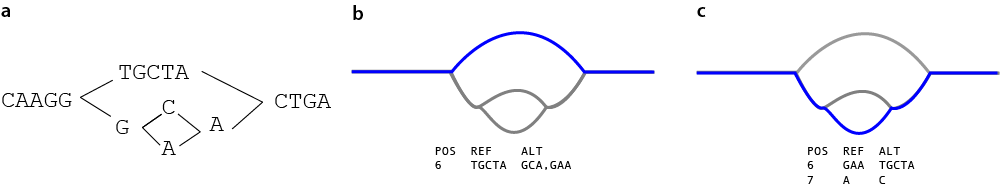
\includegraphics[width=0.95\columnwidth]{Chapter0/Figs/map_variation_representation.png}
        \centering
        \caption{Single-sample variation inference}
        \label{fig:map-var-representation}
        \source{\cite{rachelthesis}}
     \end{subfigure}
     \begin{subfigure}[b]{0.95\textwidth}
         \centering
        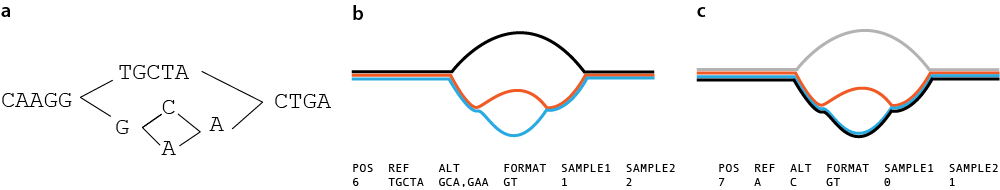
\includegraphics[width=0.95\columnwidth]{Chapter0/Figs/variant_representation.png}
         \caption{Multi-sample variation inference}
         \label{fig:var-representation}
         \source{\cite{rachelthesis,pandora}}
     \end{subfigure}
     \caption{The impact of sequence inference choice on variant representation. In both \textbf{(a)} and \textbf{(b)} the left panel (a) shows the \prg{}. \textbf{a)} the blue line indicates the inferred sequence (maximum likelihood path). b and c show how the choice of this sequence effects the representation of variant sites when genotyping. \textbf{b}) the black line indicates the multi-sample inferred sequence, while the blue and orange lines are two different samples. b and c show that by inferring the sequence that is maximally close to the two samples (c), small differences between the samples are represented as small variants.}
     \label{fig:pandora-var-representation}
\end{figure}

\hspace{0.75cm}

\noindent
The \pandora{} method addresses the main limitations of existing genome graph approaches (\autoref{sec:graphs-existing}) in the context of bacterial pan-genomes. In particular, \pandora{} supports both short (Illumina) and long (\ont{}) sequencing reads and removes hard reference bias by letting go of locus ordering and genotyping loci regardless of their genomic context.

Despite these advantages, there is a key limitation to the method: an inability to detect novel variants. As variation inference is done by genotyping all sites in a \prg{}, it follows that if a variant does not exist in a \prg{}, it cannot be detected by \pandora{}. The first chapter of this thesis (\autoref{chap:denovo}) will remove this limitation. 

% =============================================
\section{\ont{} sequencing}
\label{sec:intro-ont}
The idea of sequencing DNA and RNA with a nanopore was conceived of by multiple parties in the 1980s \cite{Deamer2016}. However, it wasn't commercially available until the release of the Oxford Nanopore Technologies (ONT) MinION\textsuperscript{\texttrademark} device in 2014 \cite{Quick2014,Deamer2016}. (We use \emph{\ont{}} sequencing to mean sequencing with an ONT device throughout this thesis). The MinION device is smaller than a smartphone and plugs into a computer via a USB port.

\ont{} sequencing works by passing a strand of DNA or RNA through a nanopore. The nanopore is embedded in an electro-resistant membrane, with a flow cell containing an array of such pores. A sensor attached to each nanopore records the electrical current passing through it; as the DNA or RNA strand moves through the nanopore, this current signal changes. There is approximately five nucleotides present in the nanopore at a time. As such, the identity of each nucleotide (base) can be inferred by a characteristic signal alteration (see \autoref{fig:nanopore}). Because the sensor takes measurements at a faster speed than the DNA moves through the nanopore, multiple recordings are obtained for each base transition - see the distinctive "steps" in \autoref{fig:nanopore}b. The process of inferring a DNA or RNA sequence from this raw signal is called basecalling.

\begin{figure}
\centering
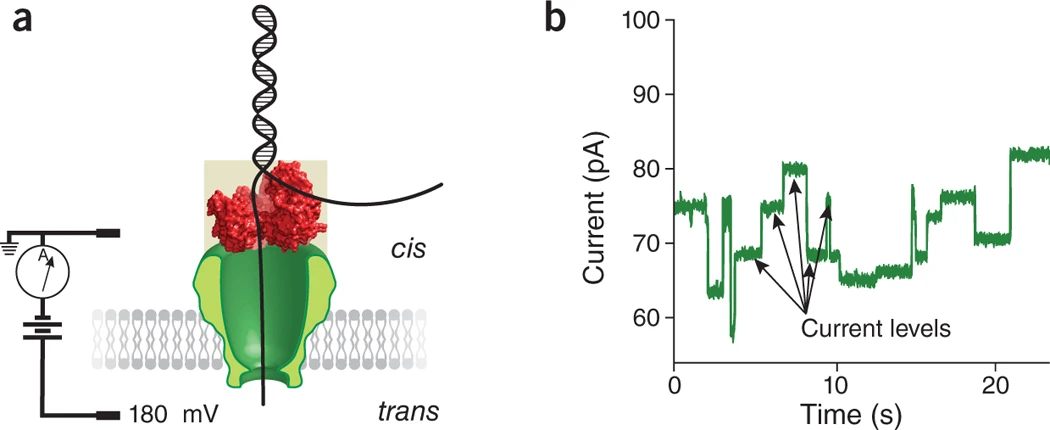
\includegraphics[width=0.9\columnwidth]{Chapter0/Figs/nanopore.png}
\caption{Nanopore sequencing. \textbf{a}) A single strand of DNA or RNA (black) is passed through a nanopore (green) by an enzyme (red). A sensor records the electric current flowing through the nanopore. \textbf{b}) The raw signal recorded by the nanopore sensor. The electrical current (y-axis) changes as nucleotides move through the nanopore. Each nucleotide can be inferred by a characteristic alteration in the signal, indicated by the black arrows.}
\label{fig:nanopore}
\source{\cite{Deamer2016}}
\end{figure}

\subsection{Basecalling}

Basecalling algorithms have seen a rich evolution since the release of ONT's first device. The raw signal and metadata for each molecule that is read by each nanopore in a flow cell is deposited into a hierarchical data format (HDF5; \cite{hdf5}) file (referred to as a fast5 file). These fast5 files are produced in real-time. That is, the user has immediate access to the sequencing data as soon as it is produced; a major benefit over existing sequencing technologies.

The progression of basecalling algorithms, along with nanopore structure and chemistry, has lead to a steady increase in the accuracy of genomic sequences inferred from \ont{} sequencing (as shown in \autoref{fig:nanopore-timeline}) \cite{Rang2018}. From initial read-level accuracy of approximately 60\% \cite{Goodwin2015}, recent studies have reported an accuracy of 93.2\% \cite{Silvestre2021}.

Traditionally, there were two key components to basecalling. The first was segmentation of the raw signal into "events" (the plateaus in \autoref{fig:nanopore}). These events represent a 5-mer within the nanopore, so consecutive events describe a sequence of nucleotides entering and leaving the nanopore. The second component to traditional basecalling is applying an algorithm to these events to infer the genomic sequence. These basecalling algorithms require an \textit{a priori} model that has been trained on molecules for which the sequence is known. Metrichor was the original software provided by ONT for basecalling and it used a hidden Markov model (HMM) to turn events into sequence. In 2017, Boža \etal{} developed the first basecalling algorithm to use a recurrent neural network (RNN), instead of a HMM, to turn events into sequence with increased accuracy \cite{deepnano}. RNN basecalling was provided soon after this with ONT's new Albacore algorithm. The next major algorithmic development was the removal of the segmentation step (the most error-prone stage of basecalling), using a Connectionist temporal classication (CTC) decoder to label unsegmented raw signal and subsequent basecalling with an RNN and convolutional neural network \cite{chiron2018,Stoiber2017}. Again, very soon after this, ONT released a new basecalling software, Guppy, which incorporated these new ideas. Guppy is still the gold-standard basecalling algorithm and all algorithmic development since its release has been related to the labelling of the raw signal data.

\begin{figure}
\centering
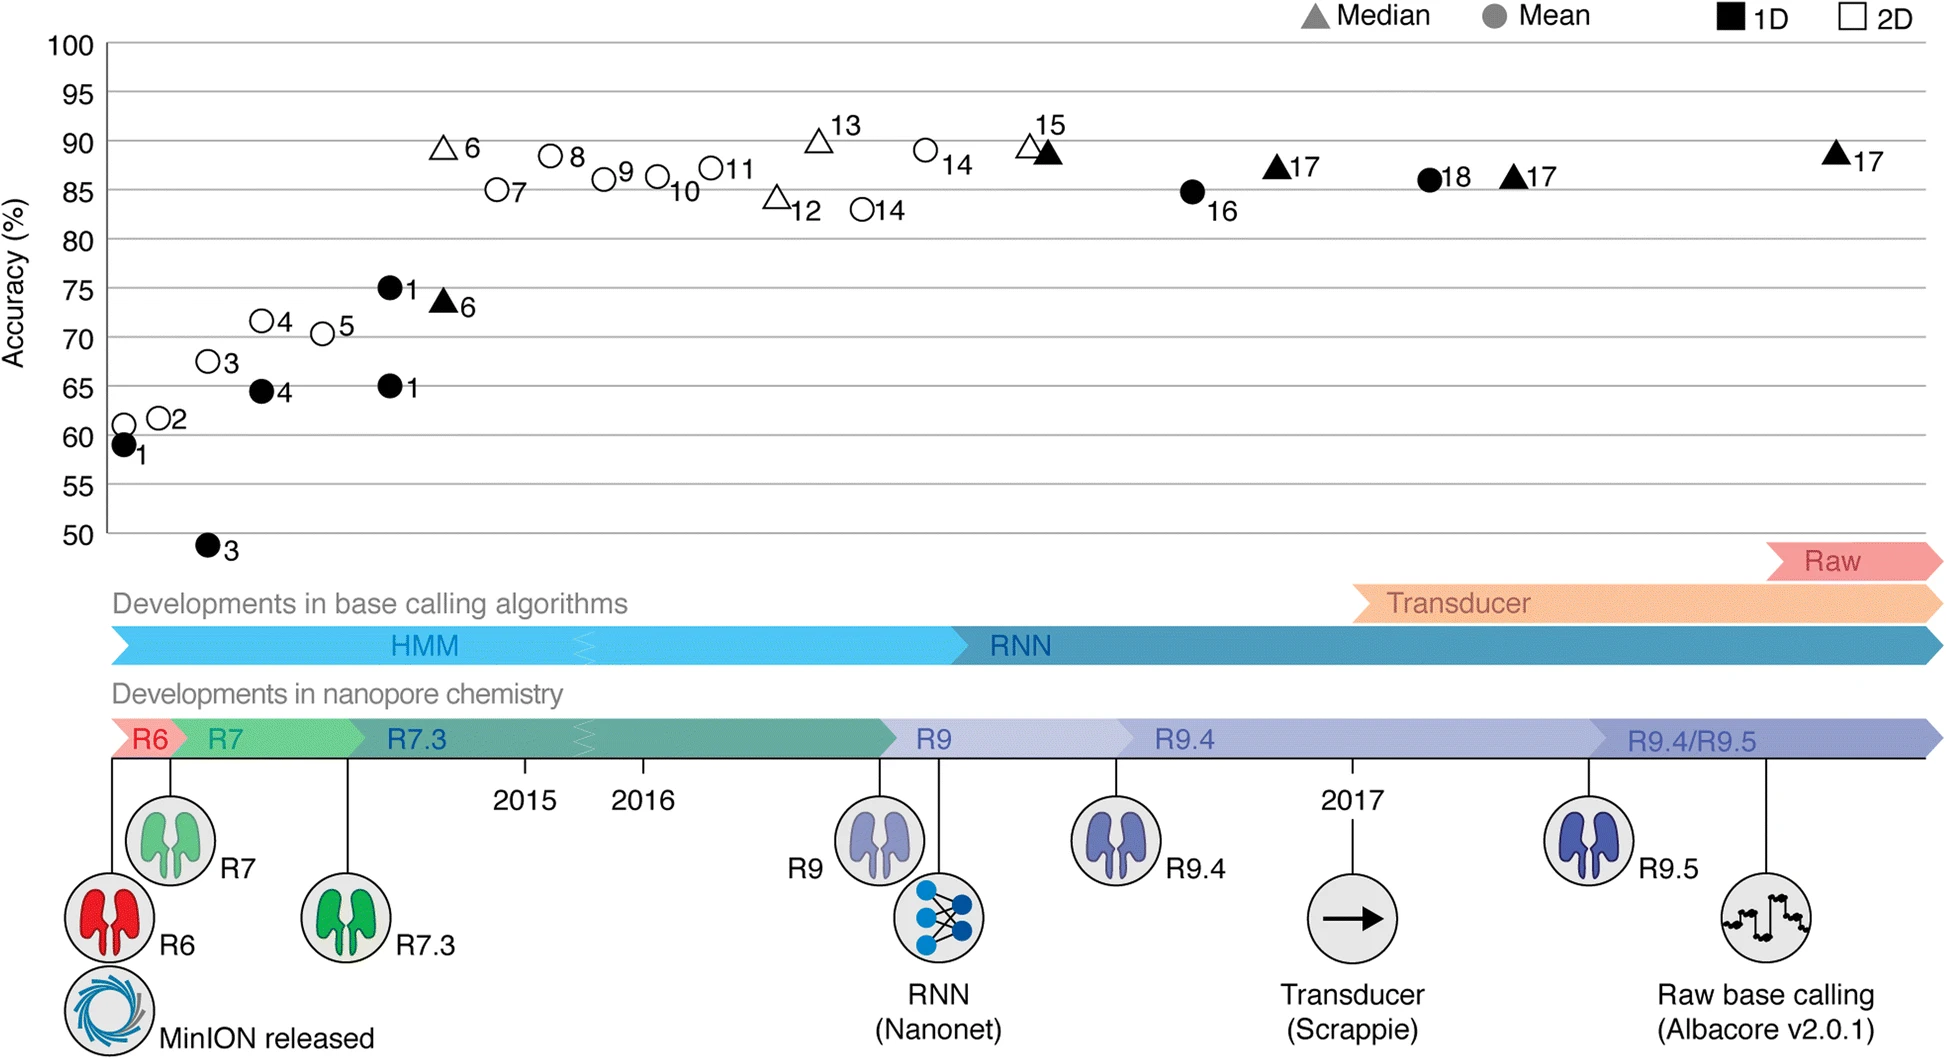
\includegraphics[width=0.9\columnwidth]{Chapter0/Figs/nanopore_timeline.png}
\caption{Timeline of ONT nanopore chemistry and the accuracy of \ont{} sequencing data. The numbers attached to each point in the accuracy plot relate to published work reporting the accuracy measurement. A list of those publications can be found in the original article this figure was taken from \cite{Rang2018}. HMM=hidden Markov model; RNN=recurrent neural network; 2D=a form of \ont{} sequencing where both strands are sequenced.}
\label{fig:nanopore-timeline}
\source{\cite{Rang2018}}
\end{figure}

\noindent
The pre-trained models distributed with \guppy{} aim to be general. That is, they can be used on \ont{} data from any organism. It is not known what species these models were trained with, however, it is fair to assume a diverse range were used given \guppy{}'s consistent performance across kingdoms and species. In 2019, Wick \etal{} showed that training a taxon-specific (Enterobacteriaceae) basecalling model can provide increased accuracy when used to basecall a sample from that taxon \cite{wick2019}. Their analysis also revealed that - at least in Enterobacteriaceae - Dcm-methylation sites were the primary source of \guppy{} basecalling errors, and that the taxon-specific model removes nearly all of the errors of this type. In addition, as has also been described elsewhere \cite{watson2019}, homopolymer deletions were found to be the next most common source of systematic errors and were also reduced with the use of a taxon-specific model.

The current state of \ont{} basecalling suggests that improvements in accuracy will come from three areas: chemistry, basecalling algorithm, and training data improvements. In \autoref{chap:tubby} we will look to improve \ont{} accuracy by focusing on the latter of those areas and training a \emph{species}-specific basecalling model.

\subsection{Variant calling}
\label{sec:ont-var-calling-intro}

Calling variation between \ont{} sequencing data and a reference genome is slowly maturing, but is yet to reach the standards set by other sequencing technologies. Much of the problems relate to the lower read accuracy of \ont{} data compared to Illumina and PacBio. A higher error rate means it is much harder for genotyping models to distinguish genuine variants from technology-derived errors.

The first method specifically designed to call variation from \ont{} data was Nanopolish \cite{nanopolish2015,nanopolish2017} - developed in 2015. It maps the raw signal for each read to the reference genome variants are to be called against, and uses a HMM to determine if the reads show support for a variant. However, Nanopolish requires access to the fast5 files in order to call variants, and this contributes to observed runtimes in the order of days and peak memory in the 100's of gigabytes \cite{clairvoyant2019}. More recent variant callers designed to support \ont{} data such as DeepVariant \cite{deepvariant}, Clairvoyent \cite{clairvoyant2019} and Clair \cite{clair2020} all use multi-layer neural networks and require significant effort on behalf of the user to operate \cite{sanderson2020}. An ONT-developed variant caller (and sequence correction) tool, Medaka (\url{https://github.com/nanoporetech/medaka}), also uses neural networks, but is much simpler to use. In addition to these newer, complex methods, some researchers have found more traditional short-read approaches such as GATK \cite{Poplin2018} can be tuned to work well with \ont{} data \cite{greig2021,bainomugisa2018,Greig2019}.

Despite the wealth of \ont{} basecalling \cite{wick2019} and assembly \cite{wick2020} benchmarking studies, there is relatively few independent variant calling assessments. A recent analysis by Sanderson \etal{} evaluated Clair, Nanopolish, and Medaka for variant calling in \textit{Neisseria gonorrhoeae} \cite{sanderson2020}. However, this study used Illumina as the "truth" and only assessed SNP calls. They found Clair was the best performing method and was able to detect 94-98\% of Illumina SNP calls, however, it required training a random forest classifier to achieve this result. In addition, in order to reduce false positive SNPs from 49-289/genome to 4-19/genome, SNP detection dropped to 76-94\%. Therefore, it remains to be seen what the true precision and recall of \ont{} variant calling is - for both SNPs and indels.

\subsection{Benefits and limitations}
\label{sec:ont-benefits}

\ont{} sequencing offers many unique benefits over the gold-standard Illumina as a result of its vastly different approach to sequencing. However, there are limitations and \ont{} will unlikely ever be a solution for all problems. We will briefly summarise some of these pros and cons in the context of pathogen genomics and its application to real-world settings with respect to Illumina.

\subsubsection{Cost}
Depending on the context of the application, \ont{} sequencing is both more and less expensive than Illumina sequencing. At a purely device and peripherals level, there are a few layers of cost that need to be understood. The upfront price of an ONT MinION device is \euro900, while an Illumina MiSeq costs \euro100,000 - 111 times more than the MinION \cite{Tedersoo2021}. The cost per lane/flow cell and library prep is \euro600 and \euro90-130 for the MinION, while for the MiSeq these two items are \euro2,000 and \euro50-100 respectively. Taking all of these prices into account, the cost of generating one billion bases (1gbp) of sequencing data is \euro12 on a MinION device and \euro175 for a MiSeq. However, the caveat here is that, currently, the 1gbp of Illumina data will be of much higher quality. Other costs that are harder to quantify are the need for longer library prep for Illumina sequencing, thus there are additional costs associated with this \cite{Tedersoo2021}.

\subsubsection{Portability}
The ONT MinION weighs just 87g and has a volume of 80cm\textsuperscript{3}, while the Illumina MiSeq respective weight and volume are 57.2kg and 202,709cm\textsuperscript{3}. The MinION can also be powered through the USB port of a computer, while the MiSeq requires significantly more power resources \cite{Tedersoo2021}. These two aspects combine to make the MinION extremely portable and the MiSeq completely stationary.

\subsubsection{Diagnostics}
Another benefit of \ont{} sequencing is that the data is made available in real-time. A standard MiSeq runtime is approximately 55 hours \cite{Tedersoo2021} and therefore it takes at least 55 hours to have access to the sequencing information. As such MinION diagnostics can operate as rapidly as the sequencing. Indeed, \ont{} sequencing has been applied to same-day \mtb{} diagnostics, with phylogenetic placement and full drug susceptibility profiles in 12.5 hours \cite{Votintseva2017}. Other real-time diagnostic applications have included detection of surgical device infections \cite{Sanderson2018}, Ebola \cite{Hoenen2016,quick2016} and Zika \cite{faria2016} virus outbreak surveillance, and Enterobacteriaceae strain and drug resistance identification \cite{Cao2016}. Even conventional genomics for bacterial diagnostics stand to gain from the use of \ont{} sequencing. For example, Greig \etal{} from Public Health England found that the better resolution of the Shiga toxin-producing \ecoli{} accessory genome from \ont{} sequencing lead to improved resolution during outbreak investigation \cite{greig2021}.

Another emerging benefit of \ont{} sequencing is the artificial enrichment of samples \cite{Payne2021,Kovaka2021}. This enrichment is facilitated by an API within the MinION device that allows for ejecting (rejecting) molecules from the nanopore. The sequencing data is mapped to a reference database and rules can be provided that reject a molecule if it originates from a specified reference, or once a certain read depth has been reached. One application by Kovaka \etal{} was to deplete bacterial DNA, thus enriching yeast genetic material \cite{Kovaka2021}, however, this could easily be employed in the reverse, depleting human DNA and enriching bacterial or viral material in a patient-derived sample.  

\hspace{0.75cm}

\noindent
While there are many benefits to \ont{} sequencing, the accuracy of data provided is still well behind Illumina. However, as we have seen, increased algorithm and method development is helping to reduce the difference. A major focus of this thesis is the improvement of \ont{}-derived sequencing information. In particular, after adding the ability for \pandora{} to discover novel variants, we will turn our attention to genome graph and \ont{} sequencing applications for the pathogen \textit{Mycobacterium tuberculosis}.

% =============================================
\section{Tuberculosis and its causative agent}

% Overview of the diseases and bug. WHO stats. Kerri's paper has some good stuff
Tuberculosis (TB) is an ancient airborne disease that predominantly effects the lungs \cite{Pai2016}; evidence suggests it has been with humans since leaving Africa \cite{Wirth2008,Comas2013}. In 2019, an estimated 1.4 million people died of TB globally, and over 10 million fell ill to the disease; 206,030 of those cases were multi-drug resistant (MDR) \cite{who2020}. The causative agent of TB is principally the bacteria \textit{Mycobacterium tuberculosis}, which has no known reservoir other than humans \cite{Comas2013}. However, other members of the Mycobaterium tuberculosis complex (MTBC), such as \textit{M. africanum}, can also cause TB \cite{Pai2016}. 

TB is a preventable and curable disease; 85\% of patients with active disease can be successfully treated with a 6-month drug treatment that has the added benefit of preventing transmission \cite{who2020}. It has been estimated that 60 million TB-caused deaths have been avoided since 2000. Despite this, TB remains in the top 10 causes of death world-wide \cite{who2020}. As a result, in 2015, the World Health Organization (WHO) and United Nations developed the End TB Strategy which aims to reduce TB deaths by 95\% of 2015 levels by 2035 (among other goals) \cite{endtb2020}. One of the major pillars of the End TB Strategy is "Intensified research and innovation" through the "discovery, development and rapid uptake of new tools, interventions and strategies." Another pillar, which will be a major focus of this thesis, is improved patient-centred diagnostics for the "early diagnosis of tuberculosis including universal drug-susceptibility testing, and systematic screening of contacts and high-risk groups."

\subsection{Epidemiological and phylogenetic diagnostics}
Public health applications for whole genome sequencing (WGS) of \mtb{} generally focus on three diagnostic use-cases: species/lineage identification, prediction of drug resistance, and clustering of samples for epidemiological purposes \cite{Gordon2021,Meehan2019}.

\subsubsection{Species/lineage identification}
The MTBC is composed of seven species of Mycobacteria with varying growth, host, and pathology characteristics \cite{Homolka2012}. In addition, non-tuberculous mycobacteria (NTM), such as \textit{M. abscessus} and \textit{M. avium}, can cause infections that present similarly to those of the MTBC \cite{Johansen2020}. However, NTMs can have very different drug resistance profiles to MTBC members \cite{Floto2016,Johansen2020}, highlighting the importance of correct species and lineage identification.

Routine species and lineage identification for suspected TB cases involves the use of the GenoType CM and AS line probe assays (LPA; Hain Lifescience) \cite{Makinen2006,Quan2018}. These LPAs works by reverse hybridisation of PCR products from the sample to species-specific probes from the 23S rDNA region \cite{Makinen2006}. In contrast, the resolution provided by WGS means that the various lineages and species can be delineated in a single test, and can be easily adapted to new markers or lineages/species. WGS identifies species and lineage by detecting SNPs known to be unique to each species, lineage, and sublineage \cite{Coll2014,Homolka2012,Stucki2016standard,Lipworth2019,Freschi2020}, and has been proven as accurate enough for adoption by Public Health England \cite{Quan2018}.

\subsubsection{Transmission cluster detection}
The inference of possible transmission events is an important component of preventing ongoing TB infections. Given the low mutation rate in \mtb{} - 0.5/SNPs/genome/year \cite{walker2013} - clustering tends to work off the assumption that samples with few SNP differences are likely part of a transmission event. 

Until recent, the mycobacterial interspersed repetitive-unit–variable-number tandem-repeat (MIRU-VNTR) genotyping was the primary method for TB outbreak investigation \cite{walker2013}. MIRU-VNTR is a PCR test that measures the size of tandem repeats (VNTRs) from 24 loci in the \mtb{} genome. The size of these VNTRs, as the name suggests, is variable among strains, and so this can be used to \emph{exclude} transmission. However, without epidemiological data in support, it is unable to provide the fine-grained information needed to infer likely transmission \cite{walker2013,Wyllie2018}.

Illumina WGS has been extensively validated as a preferred means of identifying \mtb{} genetic relatedness - at least in high-income settings \cite{Gardy2011,walker2013,Wyllie2018,tbmask2014,Hatherell2016}. It provides greater resolution and lower costs than MIRU-VNTR, and is now routinely used in some public health agencies, such as Public Health England \cite{Wyllie2018}. Clustering samples based on WGS data is done by first calling SNPs with respect to the \mtb{} reference genome. The number of SNP differences between two samples defines their genetic distance (or relatedness). Second, the pairwise distances for all of the samples under investigation are used to cluster cases if they have a distance less than or equal to a predefined threshold \cite{Gardy2011,walker2013}. For example, if the threshold is set to 5 and two samples $A$ and $B$ have a distance of 4, they are considered part of the same cluster. If a third sample $C$ has a distance of 6 from $A$, but 2 from $B$, $C$ is added to the cluster. Further epidemiological information can also be incorporated to improve connections \cite{Gardy2011}.

Two main problems that afflict WGS-based clustering are bioinformatic and threshold disparity. The method for obtaining SNPs for a sample is far from standardised. The consequence of this lack of consistency was masterfully demonstrated by Walter \etal{} when they asked five different genomic epidemiological research groups to produce variant calls from the same outbreak data \cite{walter2020}. They found these variant call sets did not produce consistent transmission inferences and found that filtering of variants had a noticeable negative effect. Furthermore, an eminent study from Stimson \etal{} recently highlighted the issues with SNP threshold-based WGS clustering \cite{stimson2019}. These limitations come down the variety of SNP thresholds and the contexts in which they are calibrated \cite{stimson2019}. They provide an alternative approach that uses SNP difference, timing of cases, molecular clock rates and transmission processes to produce clusters based on the probability of two cases being separated by a given threshold of transmission events.

In addition to the limitations just described, \ont{} WGS for transmission inference has yet to see a thorough investigation. Smith \etal{} recently assessed \ont{} sequencing against Illumina but provided very little detail about the clustering and only used a small portion of their data for assessing clusters. This shortcoming motivates the work in \autoref{chap:clustering} where we examine \ont{}'s ability to produce transmission clusters concordant with Illumina.

\subsection{Antimicrobial resistance prediction}
Antimicrobial resistance (AMR) is a global concern for TB care and prevention. The End TB Strategy seeks universal access to drug susceptibility testing (DST). The first-line drugs used in TB treatment are isoniazid, rifampicin, pyrazinamide, and ethambutol, while second-line antimicrobials include fluoroquinolones and aminoglycosides. \mtb{} that is resistant to rifampicin (RR-TB) and isoniazid are deemed multi-drug resistant (MDR-TB). These two drugs are the most effective available, so their detection is crucial in reducing the global TB burden \cite{who2020}. In 2019, it was estimated that 3.3\% of new TB cases, and 18\% of treated cases, were MDR-TB or RR-TB, with 78\% of RR-TB also being MDR-TB \cite{who2020}.
%  taken from TAC3 report
Traditionally, TB standard of care required phenotypic testing of the infecting organism against the four first-line drugs to ensure that appropriate treatment is prescribed. However, \mtb{} is a slow-growing organism, thus phenotypic testing takes many weeks to complete and can delay correct treatment by up to 80 days \cite{Pankhurst2016}. Thankfully, the Xpert\textregistered MTB/RIF assay (Cepheid) has helped provide rapid RR-TB testing (and TB detection), and in 2019, 61\% of confirmed TB cases were tested for rifampicin resistance. The Xpert\textregistered MTB/RIF assay is a PCR test that simulatenously detects MTBC and known rifampicin resistance-causing mutations in the \textit{rpoB} gene in as little as two hours \cite{Boehme2011}. In addition, the newly developed and tested Xpert\textregistered MTB/XDR (Cepheid), which tests for resistance to isoniazid, fluoroquinolones, ethionamide, and aminoglycosides \cite{Cao2021}, stands to provide much greater access to diagnostics \cite{Bainomugisa2020}.

These Xpert\textregistered assays are a welcome addition to DST of TB. However, due to their (necessary) use of a fixed set of resistance-causing genotypes, drug susceptibility cannot be inferred \cite{Sanchez2015}. This inflexibility was highlighted in 2015, when 30\% (38/125) of phenotypically RR-TB in Swaziland were deemed not RR-TB by the Xpert\textregistered MTB/RIF assay, due to the presence of \textit{rpoB} mutation I491F \cite{Sanchez2015}. As a result, the Xpert\textregistered MTB/RIF could not be reliably used in Swaziland, or any other country with this RR-TB population.

WGS offers a more flexible solution that is much faster than gold-standard phenotyping methods - and now cheaper \cite{Pankhurst2016,Votintseva2015,Votintseva2017}. In addition, the accuracy of WGS-based predictions is now comparable to phenotyping \cite{hunt2019,walker2015,bradley2015,Pankhurst2016,Votintseva2015}, and can even be used as a replacement for first-line drug DST \cite{cryptic2018}. 

Predicting drug resistance from WGS data typically works by detecting the presence of known resistance-causing mutations from a curated catalogue. The two most commonly used open-source software programs for WGS AMR prediction are TBProfiler \cite{coll2015,phelan2019} and Mykrobe \cite{bradley2015,hunt2019}; although, in-house custom scripts are also prevalent \cite{smith2020,cryptic2018}. TBProfiler uses an alignment-based variant calling pipeline (\autoref{sec:aln-var-call}) to identify the presence of mutations in their catalogue. Mykrobe, on the other hand, takes an assembly-based approach (\autoref{sec:asm-var-call}) and maps reads to de Bruijn graphs built from \textit{in silico} probes of catalogue mutations. 

Previous assessments of WGS-based AMR prediction for TB have focused on Illumina sequencing. However, as we saw in \autoref{sec:intro-ont}, \ont{} provides greater speed to results, reduced costs, and portability of sequencing. Indeed, proof-of-concept work by Votintseva \etal{} found it took 44 and 16 hours to gain WGS AMR predictions from Illumina's MiSeq and MiniSeq instruments, respectively \cite{Votintseva2017}. In contrast, \ont{}-based predictions were available in 12.5 hours; the technology has improved significantly since then so this time is likely to have reduced. Both TBProfiler and Mykrobe support \ont{}, however, both used a small sample size (Mykrobe n=5 and TBProfiler n=3). Recent work from Smith \etal{} confirmed the feasibility of \ont{} WGS for TB AMR prediction on a much larger, but homogeneous, cohort (n=431) with an in-house script \cite{smith2020}.

To-date, the most influential factor in the accuracy of a method's AMR predictions has been the catalogue \cite{hunt2019}. These catalogues are constructed by aggregating mutations from large cohort studies where the impact of individual mutations is linked to a phenotype \cite{hunt2019,miotto2017,phelan2019}. These catalogues have expanded significantly in recent years due to the work of the \emph{Comprehensive Resistance Prediction for Tuberculosis: an International Consortium} (\cryptic{}), who sequenced 10,290 isolates with phenotypic information for a variety of first-line drugs \cite{cryptic2018} with more samples and drug phenotypes to come \cite{Votintseva2015}. In addition, the WHO have recently released a catalogue of mutations with associated figures for their association with resistant and susceptible isolates, along with a confidence grading \cite{whopanel2021}.

\noindent
While WGS catalogue-based AMR predictions provide significantly more flexibility than molecular assays, current approaches do not detect off-catalogue mutations. As in the example with Xpert\textregistered MTB/RIF in Swaziland \cite{Sanchez2015}, if a novel mutation arises in a population, current WGS methods will not identify the resistance. The \cryptic{} consortium recently introduced a new approach whereby if an unknown mutation is identified in a gene known to be involved in resistance, they refuse to make a call and instead send the sample for phenotyping \cite{cryptic2018}. On their 10,000-odd samples, this achieved a specificity and sensitivity for first-line drugs that was acceptable for clinical usage. This method is now in use at Public Health England for all \mtb{} samples in England. Additionally, Hunt \etal{} quantified the cost of the pure-genotyping approach of \mykrobe{}, showing that 2.4-4.6\% of resistant samples were missed. 


\noindent
The lack of sufficient \ont{} WGS validation for TB AMR prediction, along with the inability for current methods to detect off-catalogue mutations, motivate the work in \autoref{chap:dst}. In this chapter, we will leverage the new \denovo{} variant discovery from \autoref{chap:denovo} to develop an AMR prediction method that uses \pandora{} and can flag off-catalogue mutations.

\subsubsection{Using genome graphs for drug resistance prediction}
\label{sec:genome-graphs-dst}
As a brief aside we introduce the benefits of \pandora{} over \mykrobe{} for the task of AMR prediction; the focus of \autoref{chap:dst}. \mykrobe{} uses population genome graphs built from a catalogue of known resistance-causing mutations for the genotyping of samples. The underlying method \mykrobe{} uses for this is Cortex \cite{iqbal2012} - an assembly-based variant caller that uses de Bruijn graphs (dBGs; see \autoref{sec:asm-var-call}). Cortex is somewhat of a precursor to \pandora{}. However, \pandora{} offers a number of advantages over Cortex. The first being the representation of the genome graph itself. Cortex uses \kmer{}s in coloured dBGs, while \pandora{} uses minimizing \kmer{}s in a \emph{directed} acyclic graph (see \autoref{sec:make_prg}). In the context of \ont{} data, this distinction is important. Building dBGs from \ont{} data creates very complex graphs due to the number number of erroneous \kmer{}s that result from the high error rate. In addition, as the \ont{} error rate is higher than Illumina, a smaller \kmer{} size is required, another factor that increases the complexity of the dBG. Another important difference in the graph representations of Cortex and \pandora{} is the way in which \kmer{} "hits" are incorporated. In a dBG, anywhere that a \kmer{} matches, the depth is incremented by one. However, in \pandora{} such hits are dependent on the context of the read (see \autoref{sec:quasi-map}). If a \kmer{} matches two locations in the graph, but one location has many hits close by from the same read while the other does not, the spurious hit is discarded. This filtering of \kmer{} hits allows \pandora{} to use a lower \kmer{} size ($k=15$) than Cortex (\mykrobe{} uses $k=21$). Another flow-on effect of using a smaller \kmer{} size is \pandora{} does not require as much read depth as there is a much higher chance of matches to smaller \kmer{}s, especially when the error rate is high. For example, assuming a \ont{} error rate of 0.08, we would expect the probability of a $15-mer$ and $21-mer$ having no errors to be 0.30 and 0.19 respectively.


% =============================================
\section{Executive summary of this thesis}

We begin this thesis in \autoref{chap:denovo} by describing algorithms to facilitate the \denovo{} discovery of variants in a (\pandora{}) genome graph. We first calibrate this method, and associated parameters, on a simulated dataset and show that without it, \pandora{} is unable to discover any variants not present in a \panrg{}. Next, we use an empirical dataset of 20 diverse \ecoli{} genomes with Illumina and \ont{} data to evaluate the precision and recall of \pandora{}, with and without \denovo{} variant discovery. We additionally show that \pandora{}'s representation of a pan-genome as a genome graph provides superior recall to single-reference methods and a substantially lower \ont{} error rate than existing methods.

For the remainder of the thesis, we turn our attention to \mtb{} and investigate how genome graphs and \ont{} sequencing can improve public health applications for this pathogen. In \autoref{chap:clustering}, we provide a detailed analysis of \ont{}-based transmission cluster inference. Using a diverse dataset of 150 \mtb{} clinical isolates, we show that transmission clusters derived from \ont{} genetic relatedness are highly concordant with those inferred from Illumina and do not miss any samples from their expected cluster. Additionally, we explore the efficacy of \pandora{} for constructing transmission clusters and find that while no samples are missed from their expected clusters, more work is needed to prevent merging of separate clusters.

In \autoref{chap:dst}, we outline a method for drug resistance prediction with \pandora{} reference graphs (\drprg{}). We compare this method and \mykrobe{} against available first- and second-line drug phenotypes for the 150 samples from \autoref{chap:clustering}. As a result, we simultaneously show that \ont{} WGS AMR predictions are concordant with Illumina and \drprg{} predictions are consistent with \mykrobe{} - and better for some drugs. In addition, we measure \drprg{}'s ability to detect off-catalogue mutations and find that it leads to less missed resistance predictions.

Finally, in \autoref{chap:tubby}, we train an \mtb{}-specific \ont{} basecalling model and illustrate its increased read- and consensus-level accuracy over the default basecalling model. Furthermore, we show that our species-specific model reduces homopolymer deletion errors; an error type we encounter multiple times in this thesis.